\documentclass[tikz]{standalone}
\usepackage{pgfplots}
\usepackage{xcolor}
\usetikzlibrary{calc}
\pgfplotsset{compat=1.18}

\begin{document}
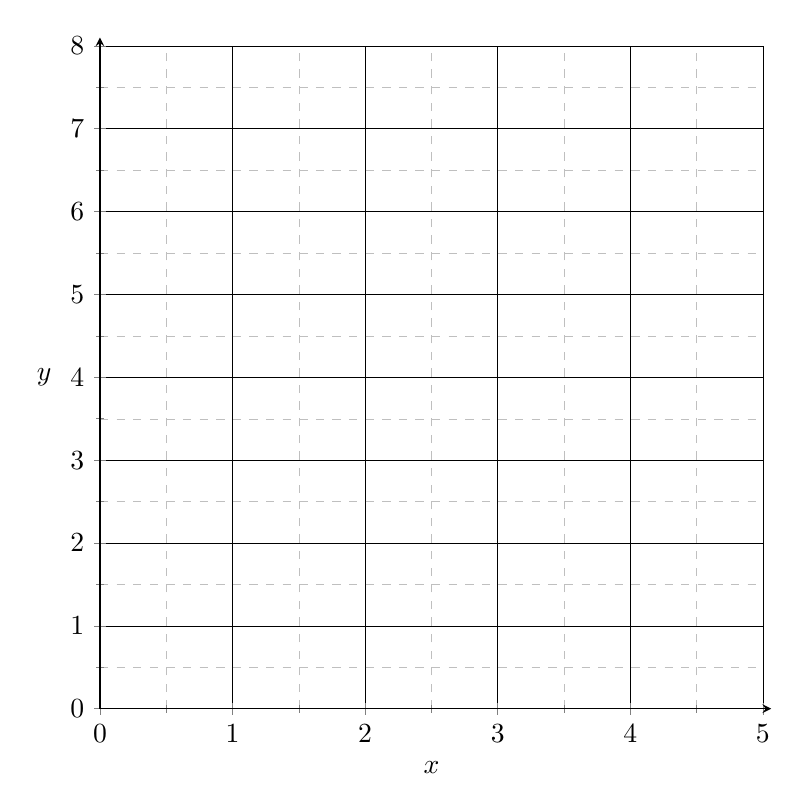
\begin{tikzpicture}
  \begin{axis}[
    axis lines=left,
    x axis line style={->,>=stealth, shorten >=-3pt},
    y axis line style={->,>=stealth, shorten >=-3pt},
    xlabel={\(x\)},
    ylabel={\(y\)},
    ylabel style={rotate=-90},
    xmin=0, xmax=5,
    ymin=0, ymax=8,
    xtick={0,1,...,5},
    ytick={0,1,...,8},
    minor x tick num=1,
    minor y tick num=1,
    grid=both,
    major grid style={line width=0.2pt,draw=black},
    minor grid style={line width=0.1pt,draw=gray!50,dashed},
    width=10cm,
    height=10cm,
  ]
    % Data points: (1,3) and (2,6)
    % Points will be added as SVG overlays for fragmentation
  \end{axis}
\end{tikzpicture}
\end{document}
